\documentclass[man,floatsintext]{apa7}
\usepackage{graphicx}
\usepackage{float}
\usepackage{todonotes}
\usepackage{longtable}
\usepackage[style=apa,backend=biber,isbn=false,eprint=false]{biblatex}
\DeclareLanguageMapping{american}{american-apa}
\addbibresource{../../.resources/biblatex.bib}
\usepackage{pgfplots}
\usepackage{xeCJK}
\usepackage{booktabs}
\title{The genes and outer stimulation that can affect the performance of basketball}
\shorttitle{EXTENDED PROJECT QUALIFICATION}
\author{Bingxin Zhao}
\affiliation{
Centre Number: 94825 \\
Candidate Number: 1032 \\
Unit Number: P301 \\
EPQ June 2024
}
\begin{document}
\maketitle
\tableofcontents
\newpage


\section{Introduction}


In the category of basketball, we used to believe that enhancing performance was all about physical training. It included team work, tactical analysis and many other things. But even though these factors definitely make basketball better, they have their own dangers too like getting hurt physically such as having a knee permanently injured, shoulder or finger or experiencing psychological damage due to being pushed too hard by the coach or bullied from teammates. This leads us to ask more questions about how genes and outside forces affect playing better in basketball. Understanding the size and strength of various external stimulations becomes even more important when we try to make plans for enhancing performance. The paper's goal is to understand how intrinsic genes and external stimulations work, comparing their importance and suggesting thoughtful methods for better basketball performance. 

\section{Literature Review}

\subsection{The intrinsic gene factors}
The game of basketball event lasts for 2 hours to 3 hours when playing 40-minute rules: four 10-minute matches in total and there are 5-minute breaks between each period. A basketball player usually plays for 40 minutes and runs about five to seven kilometers per game. Moreover, there are 1000 movements for male athletes and 650 for female athletes. An intense game may even reach 1100 discrete movements.\autocite[13-14]{raduScienceBasketball2018} As a result, basketball requires high level of endurance, explosive power and physical state for the players. Although these variables can be improved by the physical training or daily diet, your physical qualifications, which determined by the genes, can play an essential role in performing better in basketball.

As we can see from Cambridge dictionary, endurance means ``the ability to keep doing something difficult, unpleasant, or painful for a long time'' which requires a large amount of energy from the body cells to maintain the physical state. In this research, we are mainly discussing the endurance of the muscles. Including the ability to maintain the explosive power and muscle contract. People who have high endurance tend to stay in their best state for a long time. The game of basketball event lasts for 2 hours to 3 hours when playing 40-minute rules: four 10-minute matches in total and there are 5-minute breaks between each period. As a result, the players may require good endurance to maintain their physical state, especially for the muscle cells.

The reason why endurance can affect the physical state is that it affects the efficiency of aerobic respiration.\autocite{forsmanh.KoripalloilijanFyysinenHarjoittelu2024} Exercise and moving require constriction and relaxation of the muscle cells which require the energy from respiration. If the efficiency of aerobic respiration can be improved, the energy produce can increase, so that the muscle fibers can have the sufficient energy to contract and relax more regularly. Gens that are related to enzymes of energy metabolism, the raw material of the aerobic respiration and the storage of metabolites in muscles have been proved to play a role in affecting the aerobic respiration.\autocite{ahmetovGenesAthleticPerformance2016}

BDKRB gene, which is correlated with higher skeletal muscle metabolic efficiency and glucose uptake during exercise, helps to increase the amount of glucose in our body and helps to increase metabolic efficiency.\autocite{mareksawczukPolymorphismBradykininReceptor2013} \footnote{However, in this paper, the results have been tested that there's no significant relationship between the BDKRB gene and exercise. It can still be considered an influence factor due to its mechanism of action. There may also be errors in this study that cause the differences of the studies so this result should be further tested.} Another kind of gene is ACE, which is an element of renin-angiotensin system. This kind of gene is crucial for regulating blood pressure. It also maintains the water-electrolyte balance.\autocite{loefflerBiochemieUndPathobiochemie2019} Insertion of the DNA sequence of ACE is associated with increased endurance performance. The genes of the PPAR group also play an important role in the regulation of energy metabolism via mitochondria. Transcription factors of the PPAR group influence several genes involved in fat and carbohydrate metabolism and uptake of glucose into skeletal muscles \autocite{loefflerBiochemieUndPathobiochemie2019} and glucose is the raw material for aerobic respiration. These genes have shown their ability to increase the cell metabolism and the respiration, hoping to increase the endurance of the athletes.

Apart from the endurance, the efficiency of aerobic respiration is also considered as an important variable that can effect the basketball performance. Aerobic respiration is the general form for a series of reactions, which are usually described as four stages: glycolysis, link reactions, the Krebs cycle, and the chain of electron transport. Aerobic respiration is the process for all the body cells to produce ATP, the energy, in order to perform the functions like contraction and dilation of the muscles. 

In the respiration, NAD and FAD, witch are both enzymes, play irreplaceable parts. They accept the hydrogen ion from the pyruvate and donate the hydrogen ion and electron in the electron transport chain so that the electrons and hydrogen ions can produce energy when passing the protein channels. As a result, if the hydrogen ions can be carried and released effectively in a short time, the rate of producing energy will increase. Slc12a8 gene synthesis protein that helps to produce NAD. The Slc12a8 proteins carry the NMD, which is the raw material of NAD, into the cell to produce NAD. \autocite{grozioSlc12a8NicotinamideMononucleotide2019} If the Sic12a8 genes are widely expressed, the amount of NAD might increase. As a result, the cells' ability to circulate the hydrogen ions will be more efficient, so the rate of aerobic respiration increases.

There are also some genes that have been scientifically proved to have an interplay with the sports performance. ACTN3 gene is a typical example. Scientists have proved that there's a strong relationship between the ACTN3 gene and sports performance. For elite athletes, ACTN3's X and R alleles has been proved to affect the capability of sprinting and endurance. About 92\% of Olympic short-distance runners have been reported to have a gene with R section.\autocite{goelACTN3AthleteGene2007}

Last but not least, there are also some genes that influence the body qualification by affecting the muscle function, like C18ORF25. The study has shown that there's a strong correlation between the C18ORF25 gene and exercise capacity and muscle function. The C18ORF25 gene can improve and build up the skeletal muscle, which can be a huge benefit for athletes.\autocite{blazevPhosphoproteomicsThreeExercise2022}

Overall, most of the genetic reasons are inborn and cannot be changed easily. Although there are some ideas about changing the DNA base sequence of the genes like using the CRISPR/Cas9 to edit the DNA and improve the sports performance, it's not ethical and can pollute the gene pool, which cause a severe problem. What's more, the side effects from changing genes are serious. They may cause genetic diseases and strongly affect the offsprings. As a result, it's hard to perfect the basketball performance through genes, outer stimulations seem to have a more reliable way. 

\subsection{The outer stimulation}
Outer stimulation include artificial interruption and the natural condition. The natural condition includes the temperature, the whether, the altitude, the humidity and the basketball playground. They are strongly correlated to the mood and physical state of a player. However, these are hard to make a change to improve the basketball performance. The artificial interruption seems to be a more reliable way to change the basketball performance significantly. In this essay, we mainly focus on the auditory interference since the basketball players can be most directly affected by the sounds than the visual interruptions. Music has been proved to have effect on the basketball performance. In \textcite{mcleodConstructionMasculinityAfrican2009}'s essay, she proposed that the idea that music and sports, such as basketball, rely on rhythmic flow, polyrhythms and syncopations. This is because they affect the established expectation of audiences or opponents. What's more, the beats also unifies the audiences' state of mind and ``infuse them with appropriate rhythmic vitality''. However, less experiments have been carried out to support the analysis. 

Another auditory interference is the yelling from spectators. In \textcite{eptingCheersVsJeers2011}'s studies, the relationship between the behavior of the spectators and the basketball performance. The result is quite surprising that the mean of the three conditions: cheers, jeers, and silence are the same. The author explains all the players are well trained so that the outer stimulation is not significant. However, audience can affect athletes' performance both physically and mentally (e.g., see \textcite{jonesAllWorldStage2007}). That produces conflict and investigating the relationship between audiences' behavior and the performance of the players is one of my purposes. Also, the extent of the influence between cheers and jeers, between the music stimulation or spectator's stimulation will be compared. In \textcite{eptingCheersVsJeers2011}'s experiment,  the researchers compared the influence of cheers, jeers, and silence. Nevertheless, the result shows that none of them can affect the athlete's behavior. The author gave the reason that the free throw is too easy for the players.

\section{The experiment}

\subsection{Experiment plan}
Initially, the experiment is planned to investigate the effectiveness of both music and the spectators on the performance of basketball. Unfortunately, due to the limitation from the school. It's hard to find the female audiences and most male audiences are friends or classmates of the basketball players. This may cause bias because it's hard to say whether the influence on basketball performance is caused by the yelling or simply the spectator himself. What's more, most of the spectators felt embarrassed and wared to cheer or bow their classmates, make the experiment even harder to operate.

To reduce the bias from people and make the experiment more reliable, only music is investigated at last. 

The aim of the essay now is to investigate the relationship between the tempo of music and the players' basketball performance

\subsection{Samples}
10 subjects are involved. They are all high school male students aged between 14 and 16 from Shanghai Baoshan World Foreign Language School and they are the members of school basketball team. All the subjects played basketball for at least once a week and all of them have trained basketball for at least 2 years. 6 of them have trained for other sports. 4 of them have trained badminton, 2 of them have trained table tennis and 2 people have practiced fencing. 

Before the experiment, they have asked to finish a questionnaire about their mood, their sleeping time and whether they have listened to music while playing basketball. They were told that the questionnaire was part of the daily training so that the demand characteristics is reduced. They were asked to scaled their mental state from 1-10 because the initial mental state may affect the performance of basketball \autocite{liuMoodStatusResponse2023} and the average is 5.63. Sleeping time are also involved because people tend to behave differently depends on their sleeping time, and the mode time is 7 hours, which is within recommended sleeping hour according to the World Health Organization. These data suggest that most of the subjects have a normal and healthy sleeping time with a peaceful mood. So the interruption caused by extremely good d and scaled by the number of
shoots, the goal number, the stealing number and the losing number. These
standards are chosen based on the NBA scouting report.\autocite{NBAZhongGuoGuanFangWangZhanQiuYuanZiLiao2024} A behavior category is made based on these factors

\begin{itemize}
\item Number of shoots: the number of throwing ball to the basket for each player, including any ball that shoots in or not; and
\item Goal number: the numor bad mood and the lack of sleeping time can be reduced. The reliability increase.
\end{itemize}

There are 3 experimenters in this study. One of them will stand on the second floor of the school gym to record the whole match with the camera. He should stand on the second floor because it's hard to be noticed by the players and can record the whole process. Another experimenter will stand beside the field as a spectator to record the data. He will also play the music during the process

A teacher is involved in the experiment who knew all the details of the experiment but he will not tell the players. He acts as a judge to regulate the composition. He will not interrupt the players in the experiment. 

\subsection{Procedure}

Before the experiment, 3 music of different tempos were chosen based on the range of BPM, which is the measurement of music tempo. 1 lento songs (ranging between 40-60 BPM) called Merry-go-round of life by the famous musician Joe Hisaishi, 1 moderato songs (98-112 BPM) called Empty love by Lulleaux and Kid Princess, and 1 Presto songs (168-200 BPM) called Usseewa by Ado were selected as the music we played.\autocite{HelloMusicTheory2022} They all have length for about 150s to 180s. They are played at volume of 50 which is the moderate volume.

The experiment was conducted in the school basketball gym. This experiment aimed to investigate the correlation between the different tempo of music and the basketball performance. The students gather in the basketball field by chance and rolled the group evenly by themselves. The basketball match will not inform any other students so that fewer spectators are aware of the match and fewer spectators are present. During the match, any fouls will not stop the watch ensuring that the match can be finished on time and the afternoon class won't be affected.

The experimenters will arrive at the play ground 5-minutes earlier than the players to test the device and discuss with the coach to ensure the details. 

When the players arrived, they will first do a 5-minutes warming up exercise which is lead by their coach. After that, they will divide into two groups of 5 people and starting the competition as follows:

\begin{enumerate}
    \item In the first 3 minutes' competition, no music is played. 
    \item In the second 3 minutes' competition, Merry-go-round of life was played.
    \item In the third 3 minutes' competition, Empty love was played.
    \item In the last 3 minutes' competition, Usseewa was played
\end{enumerate}

There's a five-minute break between each competition. The experimenter will guide them to have a rest between each condition, involving some communication about the feelings during the process.

Each video is recorded for 10-minutes. After recording the video, the experimenter will review it and finish the behavior categories.

\begin{longtable}{@{}llllll@{}}
 \toprule
    Music type & Name & Shot & Goal & Percentage & Missing \\
    \endfirsthead
    \toprule
    Music type & Name & Shot & Goal & Percentage & Missing \\
    \endhead
    \midrule
    \endfoot
    \bottomrule
    \caption{Basketball shooting statistics under different music conditions}
    \label{basketballtable} \\
 
    \endlastfoot
        \midrule
        No music & B & 1 & 0 & 0\% & 3 \\
                 & W & 3 & 1 & 33\% & 2 \\
                 & T & 0 & 0 & 0\% & 0 \\
                 & H & 2 & 0 & 0\% & 0 \\
                 & M & 2 & 1 & 50\% & 1 \\
                 & P & 4 & 1 & 25\% & 3 \\
                 & K & 1 & 0 & 0\% & 3 \\
                 & J & 0 & 0 & 0\% & 0 \\
                 & X & 5 & 1 & 20\% & 0 \\
                 & A & 4 & 3 & 75\% & 2 \\
        \midrule
        Lento music & B & 1 & 1 & 100\% & 3 \\
                    & W & 3 & 2 & 67\% & 0 \\
                    & T & 0 & 0 & 0\% & 0 \\
                    & H & 5 & 1 & 20\% & 1 \\
                    & M & 3 & 1 & 33\% & 1 \\
                    & P & 3 & 1 & 33\% & 0 \\
                    & K & 0 & 0 & 0\% & 0 \\
                    & J & 0 & 0 & 0\% & 3 \\
                    & X & 6 & 1 & 17\% & 0 \\
                    & A & 1 & 0 & 0\% & 0 \\
        \midrule
        Moderato songs & B & 3 & 2 & 67\% & 0 \\
                       & W & 3 & 3 & 100\% & 0 \\
                       & T & 0 & 0 & 0\% & 0 \\
                       & H & 2 & 0 & 0\% & 0 \\
                       & M & 5 & 2 & 40\% & 3 \\
                       & P & 2 & 1 & 50\% & 2 \\
                       & K & 4 & 2 & 50\% & 5 \\
                       & J & 0 & 0 & 0\% & 1 \\
                       & X & 4 & 4 & 100\% & 3 \\
                       & A & 3 & 3 & 100\% & 0 \\
        \midrule
        Presto songs & B & 3 & 2 & 67\% & 0 \\
                     & W & 3 & 2 & 67\% & 0 \\
                     & T & 0 & 0 & 0\% & 0 \\
                     & H & 3 & 1 & 33\% & 0 \\
                     & M & 4 & 2 & 50\% & 1 \\
                     & P & 3 & 1 & 33\% & 2 \\
                     & K & 1 & 1 & 100\% & 2 \\
                     & J & 0 & 0 & 0\% & 0 \\
                     & X & 5 & 3 & 60\% & 0 \\
                     & A & 3 & 1 & 33\% & 0 \\

\end{longtable}

After the experiment, three players are selected randomly to have an interview. First, there will be an apology for the deception and misinformation of the experiment. The subjects were told to inform other players in the team about the experiment. Next, I will ask them whether they have expected an experiment. Then, their feeling is asked for further information.

\subsection{Measurement}
The basketball performance is operationalized and scaled by the number of shoots, the goal number, the stealing number, and the losing number. These standards are chosen based on the NBA scouting report \autocite{NBAZhongGuoGuanFangWangZhanQiuYuanZiLiao2024}. A behavior category is made based on the following factors:

\begin{itemize}
\item Number of shoots: the number of throwing balls to the basket for each player, including any ball that shoots in or not
\item Goal number: the number of balls that shoot in the basket
\item Stealing number: the time that the player ``steals'' or grabs the ball from the opponents
\item Missing number: the time that the player loses their ball because of the attack by the opponents.
\end{itemize}

\subsection{Results}

The result, as shown in table \ref{basketballtable}, shows that there's little change between the choosing number. however, there's a significant difference between the music with a higher tempo of music (X>98 BPM) and lower tempo of music (40-60 BPM) or no music. The goal number for Lento music is the same as the control group at 7 points. In the Moderato song, the goal number is the highest at 17 points, and in the Presto song, the number is a little smaller at 13 points. Figure \ref{scoring_percentage} show the average percentage for each type of song.

\begin{figure}[h]
\centering
 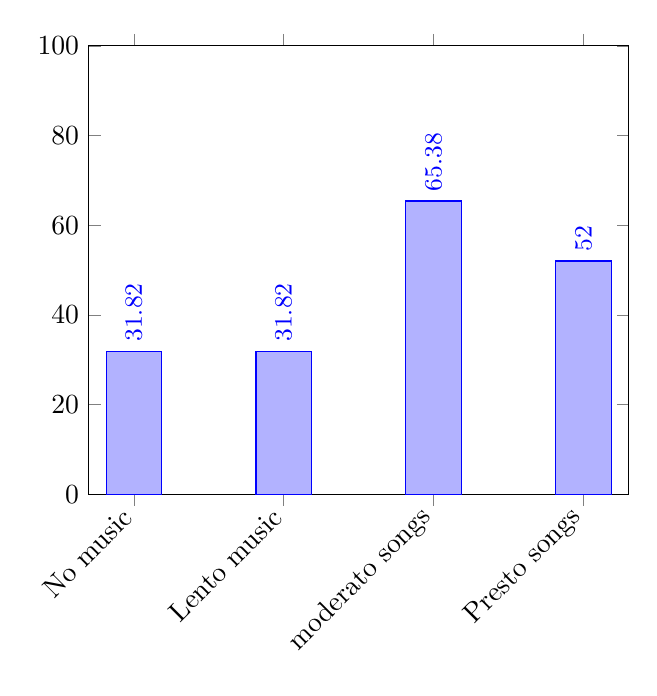
\begin{tikzpicture}
\begin{axis}[
    ybar,
    bar width=20pt,
    x tick label style={rotate=45, anchor=east},
    ymin=0,
    ymax=100,
    xtick=data,
    xticklabels={No music, Lento music, moderato songs, Presto songs},
    nodes near coords,
    every node near coord/.append style={font=\small, rotate=90, anchor=west},
    nodes near coords align={vertical},
]
\addplot coordinates {(1, 31.82) (2, 31.82) (3, 65.38) (4, 52.0)};
\end{axis}
\end{tikzpicture}   
\caption{Scoring Percentage by Music Type}
\label{scoring_percentage}
\end{figure}


As we can see in Figure \ref{scoreperc}, there's a tendency for the goal percentage for different conditions. Most players play best during the Moderato song and Presto song. Surprisingly, three players, Student J, K, and W, all reached the goal percentage of 100\% in moderato songs. There are two players that are considered to be the outliers of the study: Student T and Student M. Student T hasn't shot or gained the goal in all four conditions so his goal percentage is always 0\%. The music seemed to have no effect on Student M as his goal percentage was almost the same in all the conditions.

\begin{figure}[h]
\centering
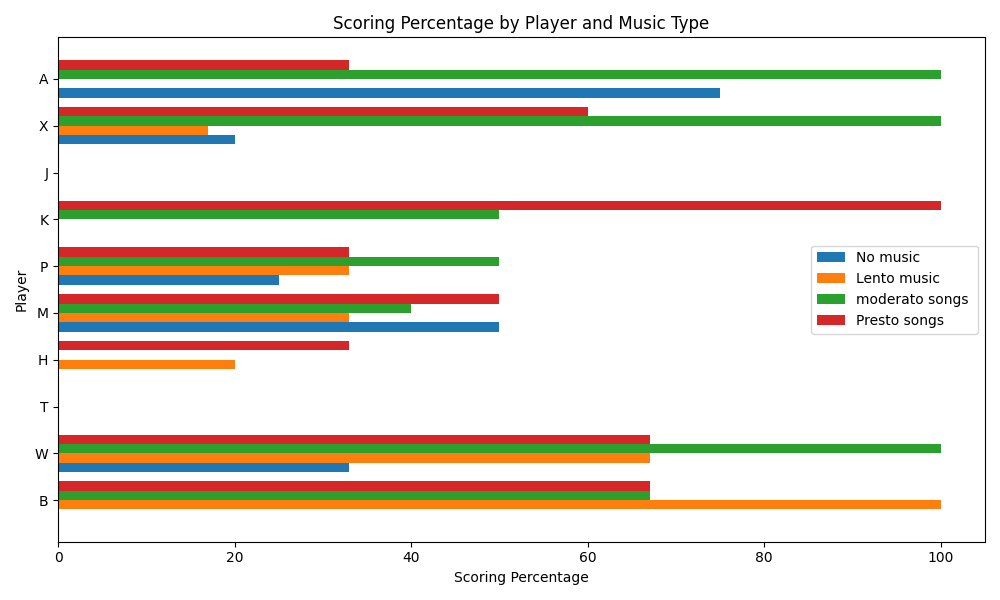
\includegraphics[width=\textwidth]{out.png}
\caption{Scoring Percentage by Player and Music Type}
\label{scoreperc}
\end{figure}

Counting the missing number is an objective way to see the concentration of the players. Only one of them, student T didn't make any mistakes during the whole process, it seemed that music didn't have any effect on him. 7 of them have an increased missing number when the music is played. However, there are also two of them, Student P and Student W, decreasing the missing number when music appeared. 

\section{Discussion}

The experiment is planned as reliable as possible. There are around 2-3 spectators around the basketball ground for each round and nearly non of them cheer or boo for the players. So the effect of the spectators' reaction has been largely reduced. Also, none of the players realized that it was an experiment, they thought that it was a little strange to have such music but no one related them to an experiment. This reduces the demand characteristics and shows that all the players have performed their real state. All the settings are placed on the same day or the same period of time, which can ensure that the mental and physical state of all the players is quite stable. The length of the rest time and competition were decided by discussing with the basketball coach, who has trained the school basketball team for more than 3 years, and during the interview, all the players thought the resting time was enough and the competition length is not so struggle. This proved that the result is less affected by their physical state, especially the errors caused by exhaustion or tiring. 

The result shows that the average goal percentage for moderato songs is the highest which reaches 50.4\%. The players get fewer goals in no music conditions compared to the conditions with music. This might explain why the rhythm of a moderato song is most similar to the rhythm of bouncing the ball for the players, providing them with the best hit for playing. In the Presto song, some players described the music as ``providing them energy'', so a pick appeared. However, for other players, the Presto song might be too ``aggressive'' or ``annoying'' so they felt uncomfortable about the music. The reason why players tended to perform worse during Lento music is that Lento songs usually have less drumbeat and they are much more peaceful. That's not fit the style of competitive sports like basketball. Nevertheless, the players thought the Lento music made them feel happy and comfortable instead of engaging them to perform better.

For the missing number, players tend to be more concentrated when Presto music is performed. The players were surprised about this result and hard to provide a possible reason. One possible suggestion is that the high speed of Presto music makes them feel ``nervous'', so they become more aware of the competition. 

7 people have increased the missing number when music is played. They complained that the music performed was so popular and familiar that they were easy to be attracted by the songs. However, 2 players tend to behave more concentrated when music is played. They suggested that they have the hobby of listening to music while doing homework. Music makes them more concentrated, so they are used to listening to music while doing other things, including playing basketball. Student T is a special outlier in this study. He was like a ``reliable passer'' so he didn't have any shooting numbers or missing numbers.

Although the experiment is tried to be as reliable with high validity. There are still some limitations that are hard to solve. First of all, the sample size is too small. The players of the basketball team are selected because they tend to perform better performing. There might be no change in different music conditions if the one was a poor player. He was unskilled in any conditions so it would be a large error. Girls are not considered in this study because of the small population. There were only 3 people who had trained and played basketball for a couple of years and that's undoubtedly insufficient for a basketball match. For these reasons, since the small sample size, the ecological validity may not be so high.

Second, the actual level of the players in the basketball team is uneven. Although they have the same training time at high school, some of them have extra sports training like table tennis, badminton, or fancy, which might improve some skills of basketball in an indirect way. What's more, the effect of training might be different. Due to the differences in their working and their attitude toward training, the training effect might be different, causing them to have differences in training skills. 

Third, the music played might also cause a bias. Three music selected, especially the Marry-go-round of Life is a classical music that is well preferred by most people. The modern song Empty Love is a popular pop song on the internet. So the reason why the players perform better might simply be the attractive music. 

Fourth, the measuring work is done by the experiment planner and another 2 students who were the classmates of the planner. The experiment has only been once so the reliability is not tested. What's more, the planner was responsible for counting the missing number which may cause a bias. Each of the experimenters was responsible for one different mission, making it impossible to make any comparison between the data recorded by several people. Although doing one experiment can decrease the chance for the players to be aware of the experiment and the order effect can also be reduced, the reliability still decreases.

Last but not least, it was hard to say 5-minutes of resting could completely overcome the tiredness caused by the matches, especially in the third or final round of study. There is a possibility that all the players feel tired after several rounds, as a result, they become less concentrated and make more mistakes in the final round, which is in the Presto music. The reliability decreases again due to this reason.

\section{Conclusion}

This essay mainly discusses the genes and outer stimulations that can affect the performance of basketball. From the genes' side, the genes can code for the proteins to increase the endurance and efficiency of aerobic respiration. To provide a more reliable suggestion for basketball players and coaches, a correlational study is set to investigate the relationship between the rhythm of music no basketball performance. The result shows that players will perform better under Moderato music (98-112 BPM) and be more concentrated under Presto songs (168-200 BPM). Although there is a lot of bias in this correlation, the conclusion can still be provided as a suggestion for the coaches and players as a support or reference to have better training or competition performance.

\section{Self-evaluation}

\subsection{Strengths}

Firstly, I have adopted a careful experiment and a variety range of papers in my dissertation. This guarantees the currency, relevance, authority, accuracy, and purpose of the data included in my article.
Secondly, I have developed a well-structured dissertation. I began by providing background information on biological factors before conducting an empirical analysis of psychological factors. Finally, I provided my own conclusions. This process ensures my clear and logical output and that all necessary content is included in the article, thus enhancing its comprehensiveness.
Lastly, I concluded my article with a feasible conclusion in reality. I believe that this project has not only improved my analytical skills but will also benefit me in my future studies. 

\subsection{Weaknesses}

First of all, as a freshman high school student, my knowledge was relatively limited. There must be gaps in my understanding of biological and psychological theory. Furthermore, I have not fully explored the feasibility of my conclusion. Some recommendations may still be ambiguous to put into practice, such as how to choose the right music for the right person. I hope I can explore it in the future.

\newpage
\printbibliography{}
\end{document}
